\chapter{Grundlagen}
Das Kapitel behandelt zuerst die Grundlagen von Reinforcement Learning.
Basierend darauf werden das Konzept des Temporal-Difference Learning und die Algorithmen Q-Learning und Sarsa erklärt.
Anschließend wird der Minimax-Algorithmus erläutert, der für die Evaluation der Agenten in der Auswertung genutzt wird.
Abschließend wird das Strategiespiel Tic-Tac-Toe erklärt.
\section{Reinforcement Learning}
Zunächst wird der Begriff Reinforcement Learning erklärt und von den anderen Teilgebieten des Machine Learning abgegrenzt.
Anschließend werden die zu lösenden Probleme und dafür genutzten Methoden formalisiert.

\subsection{Begriffserklärung und Abgrenzung}
\label{begriffserklaerung}
\acl{RL} (\ac{RL}) ist das Teilgebiet des \acl{ML}, das sich mit der Lösung von Entscheidungsproblemen beschäftigt \cite[S. 1]{suttonReinforcementLearningIntroduction2018}, \cite[S. 1]{vanderreeReinforcementLearningGame2013}.
\ac{RL} basiert auf der sogenannten \gqq{Reward Hypothese}, nach der jedes sequentielle Entscheidungsproblem als Optimierungsproblem beschrieben werden kann, bei dem der kumulierte Reward (\dt Belohnung) aller getroffenen Entscheidungen maximiert werden soll \cite[S. 53]{suttonReinforcementLearningIntroduction2018}, \cite[S. 24]{kontesg.SeminarReinforcementLearning2021}.

Das Ziel der \ac{RL} Methoden ist einen Agent zu trainieren, der eine Abbildung von Situationen auf die jeweils optimale Aktion lernt und so den Gesamtreward maximiert. 
Dem Agent wird nicht mitgeteilt, was die optimale Aktion in einer Situation ist. 
Stattdessen ist das grundlegende Paradigma von \ac{RL} Methoden, dass ein Agent mit seiner Umgebung interagiert und Erfahrung sammelt. 
Der Agent muss durch \gqq{trial and error} lernen, welche Aktionen in einer Situation gut sind und welche mit dem größten Reward verbunden ist. \cite[S. 1ff.]{suttonReinforcementLearningIntroduction2018}
Ein Beispiel der realen Welt sind Kinder, die laufen lernen. Dies erfolgt ohne Instruktionen, sondern nur durch \gqq{trial and error}. 
Richtige Aktionen werden belohnt durch Vorwärtskommen, während falsche Aktionen durch Fallen bestraft, \dahe negativ belohnt, werden. \cite[S. 289]{ertelIntroductionArtificialIntelligence2017}

\ac{RL} unterscheidet sich somit von den anderen Teilgebieten des \ac{ML}. Beim Supervised Learning (\dt Überwachtes Lernen) lernt ein Agent basierend auf einem gelabelten Trainingsdatensatz, die Abbildung einer Inputmenge auf einen Output. Ein Supervisor gibt dem Agenten instruktives Feedback, ob die beste Aktion gewählt wurde und was diese ist \cite[S. 289f.]{ertelIntroductionArtificialIntelligence2017}, \cite[S. 2]{suttonReinforcementLearningIntroduction2018}.

Ein \ac{RL} Agent muss hingegen seine Daten selbst durch Interaktion mit der Umgebung sammeln. 
Da der Agent seine Aktionen selbst wählt und seine Umgebung dadurch aktiv beeinflussen kann, sind die Daten stochastisch abhängig von den Aktionen, die der Agent zuvor getroffen hat. \cite[S. 16]{kontesg.SeminarReinforcementLearning2021} 
Zudem kann der \ac{RL} Agent kein instruktives Feedback erhalten, da sequenzielle Entscheidungsprobleme gelöst werden sollen und die Bewertung einzelner Aktionen gegebenenfalls nicht bekannt ist. 
Erst nach Erreichen \bzw Nicht-Erreichen des Ziels können die Aktionen bewertet und der Agent durch ein evaluatives Feedback belohnt werden. \cite[S. 17]{suttonReinforcementLearningIntroduction2018}
Dieses Problem des verzögerten Rewards ist ein weiteres Alleinstellungsmerkmal von \ac{RL} und bekannt als \gqq{Credit Assignment Problem} \cite[S. 17]{suttonReinforcementLearningIntroduction2018}.
Jedoch ermöglicht es die Anwendung von \ac{RL} auf Probleme, bei denen die optimale Strategie nicht bekannt ist. \cite[S. 2]{suttonReinforcementLearningIntroduction2018}, \cite[S. 16]{kontesg.SeminarReinforcementLearning2021}
Zudem unterscheidet sich \ac{RL} vom Unsupervised Learning (\dt Unüberwachtes Lernen).
Dieses verwendet zwar ebenfalls ungelabelte Daten, aber versucht darin Strukturen zu finden und somit andere Probleme zu lösen \cite[2]{suttonReinforcementLearningIntroduction2018}.

\subsection{Formalisierung des Reinforcement Learning Problems}
\label{formalisierung}

Eine Formalisierung des \ac{RL} Problems bedeutet eine Formalisierung der Reward Hypothese. 
Wie in \cref{begriffserklaerung} beschrieben, interagiert ein Agent mit seiner Umgebung. 
Alles außerhalb der direkten Kontrolle des Agenten wird zur Umgebung gezählt. 
Diese Trennung zwischen Agent und Umgebung wird als Agent-Umgebung-Schnittstelle bezeichnet. \cite[S. 47]{suttonReinforcementLearningIntroduction2018} 
Der Agent interagiert mit seiner Umgebung in diskreten Zeitschritten $t$. 
Man unterscheidet zwischen episodischen Problemen, die zu einem Zeitschritt $T$ enden und Problemen unendlicher Zeitdauer, die kein definiertes Ende haben \cite[S. 11]{suttonReinforcementLearningIntroduction2018}.\footnote{Probleme unendlicher Zeitdauer werden im Englischen als \gqq{continuous} bezeichnet \cite[S. 11]{suttonReinforcementLearningIntroduction2018}} 
Die Folge der Zeitschritte $t,t+1,...T$ wird als Episode bezeichnet \cite[S. 54]{suttonReinforcementLearningIntroduction2018}. 

Die Interaktion kann auf drei Signale reduziert werden, wie \cref{fig:rl_agent_environment_interaction} zeigt. 
In jedem diskreten Zeitschritt $t$ erhält der Agent den aktuellen Zustand $S_t \in S$ der Umgebung. 
Auf Basis dieser Beobachtung wählt der Agent eine Aktion $A_t \in A$. 
Im nächsten Zeitschritt erfährt der Agent, wie die Umgebung auf seine Aktion reagiert durch ein Tupel $(S_{t+1}; R_{t+1})$. 
Dies umfasst den neuen Zustand, in dem sich der Agent befindet und den Reward. 
Der letzte Zustand einer Episode $S_T$ wird als Terminalzustand bezeichnet. 
Der Reward ist definiert als $R_{t+1} \in \mathbb{R}$ und kann somit positiv oder negativ sein, um eine Belohnung und Bestrafung zu modellieren. \cite[S. 47 ff.]{suttonReinforcementLearningIntroduction2018}

\begin{figure}[h]
    \centering
    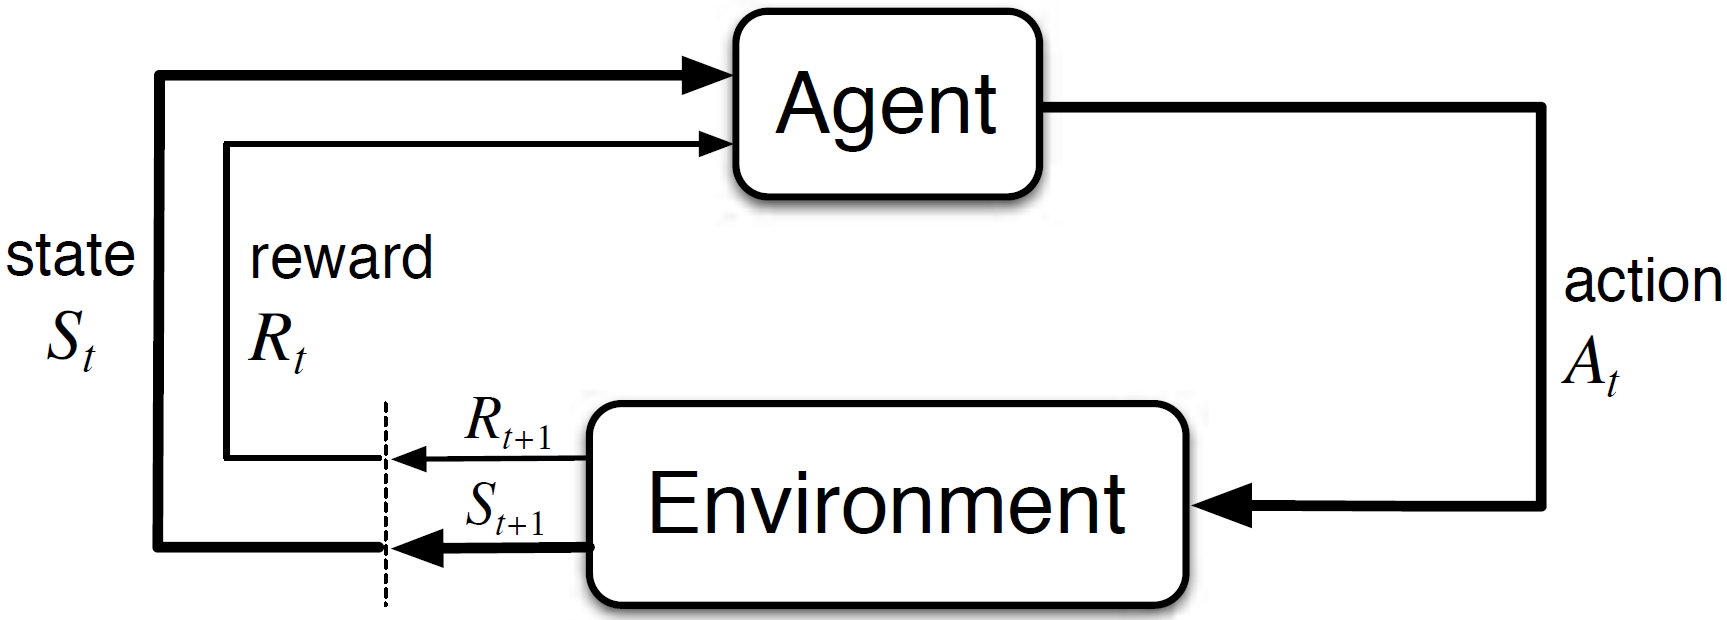
\includegraphics[scale=0.2]{04_Artefakte/01_Abbildungen/rl/rl_agent_environment_interaction.png}
    \caption[Modell der Interaktion zwischen Agent und Umgebung in einem \acs{MDP}]{Modell der Interaktion zwischen Agent und Umgebung (\engl Environment) in einem \acs{MDP} \protect\footnotemark}
    \label{fig:rl_agent_environment_interaction}
\end{figure}
\footnotetext{Abbildung entnommen aus \cite[S. 47]{suttonReinforcementLearningIntroduction2018}}

Zur Modellierung der Umgebung und deren Dynamik können \ac{MDP} genutzt werden. \ac{MDP} basieren auf  Markov Ketten und gehören zum Gebiet der mathematischen Optimierung. Ein \ac{MDP} ist definiert als ein Tupel $(S,A,p,r)$ \cite[S. 47ff.]{suttonReinforcementLearningIntroduction2018}, \cite[S. 5]{kontesg.SeminarReinforcementLearning2021}:
\begin{itemize}
    \item $S$ = Menge von Zuständen $s$
    \item $A$ = Menge möglicher Aktionen $a$
    \item $p(s' \mid s,a) = Pr(S_{t+1}=s' \mid S_{t}=s, A_{t}=a)$ für das gilt: $\sum_{a\in A}p(s'\mid s,a) =1$ \\ State-Transition Probability 
    \item $r(s,a) \rightarrow \mathbb{R}$ Rewardfunktion
\end{itemize}

Die Dynamik der Zustandsübergänge wird modelliert durch die State-Transition Probability $p$ (\dt Zustandsübergangs Wahrscheinlichkeit). 
Sie beschreibt die Wahrscheinlichkeit, bei Wahl von Aktion $a$ im Zustand $s$ in den Folgezustand $s'$ überzugehen.
Die State-Transition Probability ist als Wahrscheinlichkeitsverteilung definiert, da die Zustandsübergänge nicht deterministisch sein können. 
%Die Wahl von Aktion $a$ in Zustand $s$ kann in unterschiedlichen Folgezuständen $s'$ resultieren. 
%Die einzige Ausnahme sind Terminalzustände $S_T$, die per Definition ihr eigener Folgezustand sind \cite[S. S. 47]{suttonReinforcementLearningIntroduction2018}: $p(s \mid s,a)=1, \forall a \in A \mid S_T =s$

Zudem definiert die State-Transition Probability, dass der Folgezustand $s'$ nur vom Zustands $s$ und der darin gewählten Aktion $a$ abhängig ist. 
Zuvor besuchte Zustände oder gewählte Aktionen müssen zur Berechnung des Folgezustands nicht bekannt sein und sind implizit im Zustand $s$ enthalten. Dies wird als Markov Eigenschaft bezeichnet und ist Voraussetzung dafür, dass ein Problem als ein \ac{MDP} formuliert werden kann. \cite[S. 66]{suttonLearningPredictMethods1988}

Nach jeder Aktion des Agenten verteilt die Umgebung abhängig vom aktuellen Zustand einen Reward gemäß der Rewardfunktion. 
Die Rewardfunktion definiert das Ziel, das der Agent erreichen soll, da dieser den kumulierten Reward maximiert.
Der kumulierte Reward, den der Agent ausgehend vom Zeitschritt $t$ erhält, wird als Return $G_t$ bezeichnet. 
Für episodische Probleme ist der Return definiert als \cite[S. 54]{suttonReinforcementLearningIntroduction2018}:

\begin{equation}
    \label{eq:return_episodic}
    \equationentry{Berechnung Return $G_t$ für episodische Probleme}
    G_t=R_{t+1}+R_{t+2}+...+R_T
\end{equation}

Für Markov-Prozesse mit einer unendlichen Dauer. \dahe eine diskrete, unendliche Markov-Kette, ist $G_t$ eine unendliche Reihe, für die zur Berechnung ein Diskontierungsfaktor  $0 \le \gamma \le 1$ notwendig ist
Der Diskontierungfaktor kann auch auf episodische Probleme angewandt werden, um das Verhalten des Agenten zu beeinflussen. 
Für $\gamma=0$ beträgt $G_t= R_{t+1}$, sodass der Agent nur den direkten Reward maximiert. 
Hingegen beachtet der Agenten die späteren Rewards mit steigendem $\gamma$ mehr. \cite[S. 55f.]{suttonReinforcementLearningIntroduction2018}

\begin{equation}
    \label{eq:return_continuous}
    \equationentry{Berechnung Return $G_t$ für Probleme unendlicher Zeitdauer}
    G_t=R_{t+1}+\gamma R_{t+2}+\gamma^2R_{t+3} + \dots =\sum_{k=0}^{\infty}\gamma^{k}R_{t+k+1}
\end{equation}

Da ein Return $G_t$ den darauf folgenden Return $G_{t+1}$ enthält, kann \cref{eq:return_continuous} umgeformt werden in \cref{eq:return_nextstate}, um diese Beziehung zu verdeutlichen. Diese Beziehung aufeinander folgender Returns ist die Basis vieler \ac{RL} Methoden. \cite[S. 54 f.]{suttonReinforcementLearningIntroduction2018}

\begin{equation}
    \label{eq:return_nextstate}
    \equationentry{Beziehung aufeinander folgender Returns}
     G_t= R_{t+1}+\gamma R_{t+2}+\gamma^2R_{t+3} +\dots = R_{t+1}+\gamma(R_{t+2}+\gamma R_{t+3} +  \dots) = R_{t+1}+\gamma G_{t+1}
\end{equation}

 
Ein Beispiel für ein \ac{RL} Problem, das als \ac{MDP} modelliert werden kann, ist die sogenannte \gqq{Gridworld} in \cref{fig:gridworld_blank}. 
Der Agent startet im Feld $C1$ und soll lernen das Feld A4 zu erreichen. 
Der Zustandsraum sind die einzelnen Felder, die der Agent betreten kann. 
Das Feld B2 repräsentiert ein Hindernis und zählt nicht zum Zustandsraum. 
Die Felder A4 und B4 sind Terminalzustände. 
In jedem Zustand wählt der Agent als Aktion eine Himmelsrichtung, in der er sich bewegen möchte. Somit umfasst der Aktionsraum für jeden Zustand: Norden, Westen, Süden und Osten. 
Bei einer Bewegung in Richtung Wand oder dem Hindernis B2 verbleibt der Agent im gleichen Feld. 
Die Zustandsübergänge sind nicht deterministisch. 
Wählt der Agent eine Richtung aus, bewegt er sich nur mit einer Wahrscheinlichkeit von 80\% dorthin. 
Es besteht eine Wahrscheinlichkeit von je 10\%, dass sich der Agent in eine der angrenzenden Richtungen bewegt. 
Die Rewardfunktion definiert das Ziel des Agenten. 
Erreicht der Agent das Feld A4 erhält er einen Reward von $+1$. 
Hingegen erhält er im Agent beim Erreichen des Feldes B4 eine Bestrafung von $-1$. 
Der direkt Reward für jeden anderen Zustandsübergang des Agenten beträgt $-0,1$.
Da der Agent den Return maximiert, versucht er dadurch das Ziel in möglichst wenigen Zustandsübergängen zu erreichen. \cite[S. 10 ff.]{kontesg.SeminarReinforcementLearning2021}

\begin{figure}
    \centering
    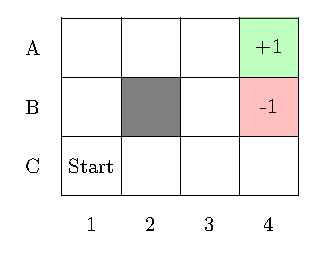
\includegraphics{gridworld/gridworld_blank.pdf}
    \caption[Aufbau des \gqq{Gridworld} Problems]{Aufbau des \gqq{Gridworld} Problems. Agent startet im Feld C1. Die Felder A4 und B4 sind Terminalzustände. B2 ist ein Hindernis.\protect\footnotemark}
    \label{fig:gridworld_blank}
\end{figure}
\footnotetext{eigene Darstellung in Anlehnung an \cite[S. 10ff.]{kontesg.SeminarReinforcementLearning2021}}

\subsection{Policy und State-Value Funktion}
\label{sec:policy_statevalue}

Der Return $G_t$ ist abhängig von den Aktionen, die der Agent in jedem Zustand wählt. 
Die Strategie, nach der Aktionen gewählt werden, wird als Policy $\pi$ bezeichnet.
Eine Policy $\pi$ ist eine Funktion $\pi(a \mid s)$, die für alle Zustände $s \in S$ die Wahrscheinlichkeit definiert, dass der Agent eine Aktion $a \in A$ wählt. 
Somit beschreibt eine Policy das Verhalten eines Agenten in jedem Zustand. 
Eine Policy kann stochastisch $\pi(a \mid s)$ oder deterministisch $\pi (s)$ sein. \cite[S. 58]{suttonReinforcementLearningIntroduction2018}

Auf der Basis einer Policy kann jedem Zustand ein Wert zugewiesen werden, der als State-Value (\dt Zustandswert) bezeichnet wird. 
Der State-Value ist der Erwartungswert des Return $G_t$, wenn der Agent im Zustand $s$ der Policy $\pi$ bis zum Ende der Episode folgt. 
Diese Abbildung von Zustand auf State-Value ist die State-Value Funktion:

\begin{equation}
    \label{eq:statevalue_function}
    \equationentry{Definition State-Value Funktion}
    v_{\pi}(s)=\mathbb{E}[G_t|S_t=s]
\end{equation}

Die State-Value Funktion kann mittels \cref{eq:return_nextstate} als Return aufeinander folgender Zeitschritte und somit aufeinander folgender State-Value Funktionen umgeformt werden:

\begin{equation}
    \label{eq:statevalue_relation}
    \equationentry{Beziehung zwischen State-Value Funktionen aufeinander folgender Zeitschritte}
    v_{\pi}(s)=\mathbb{E}_\pi[G_t|S_t=s] = \mathbb{E}_\pi[R_{t+1}+\gamma G_{t+1}]= R_{t+1} + \gamma \mathbb{E}[G_{t+1} \mid S_{t+1}=s']=R_{t+1}+v_\pi(s')
\end{equation}

\cref{fig:gridworld_policy_statevalue} zeigt für das Beispiel Gridworld eine mögliche deterministische Policy und die dazugehörige Zuweisung von State-Values. Ein Pfeil symbolisiert die Aktion, die der Agent gemäß Policy im jedem Zustand wählt. Zur Berechnung der State-Values wurde die oben beschriebene Rewardfunktion und ein Diskontierungsfaktor $\gamma=0,9$ verwendet.


\begin{figure}
    \centering
    \begin{subfigure}[b]{0.45\textwidth}
      \centering
      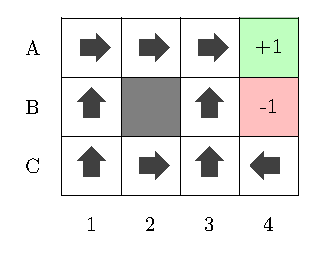
\includegraphics[]{gridworld/gridworld_policy.pdf}
      \caption{Mögliche Policy $\pi$}
      \label{fig:gridworld_policy}
    \end{subfigure}
    \begin{subfigure}[b]{0.45\textwidth}
      \centering
      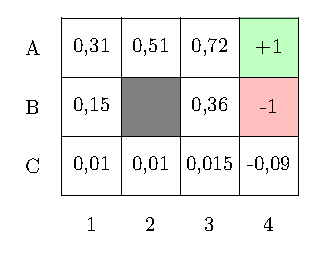
\includegraphics[]{gridworld/gridworld_statevalues.pdf}
      \caption{State-Values zur Policy $\pi$ aus (a)}
      \label{fig:gridworld_statevalues}
    \end{subfigure}
    \caption[Policy und State-Value für das Beispiel Gridworld]{Policy und State-Value für das Beispiel Gridworld\protect\footnotemark}
    \label{fig:gridworld_policy_statevalue}
    
\end{figure}
\footnotetext{eigene Darstellung in Anlehnung an \cite[S. 75.]{kontesg.SeminarReinforcementLearning2021}}

Die State-Value Funktion ermöglicht den Vergleich von Policies.
Eine Policy $\pi$ ist besser als eine andere Policy $\pi'$ wenn ihre zugehörige State-Value Funktion für alle Zustände $s$ einen größeren Wert hat, als die Policy $\pi'$: $v_\pi(s) \ge v_{\pi'}(s) \forall s \in S$

Es kann mindestens eine Policy geben, die besser als alle anderen Policies oder gleich gut ist.
Diese Policy wird als optimale Policy $\pi_*$ bezeichnet und die zugehörige Value Funktion als optimale State-Value Funktion $v_*$. \cite[S. 61 ff.]{suttonReinforcementLearningIntroduction2018}
Eine Policy ist optimal, wenn der Return $G_t$ für jeden Zustand $s \in S$ den maximal möglichen Wert annimmt.
Somit ist die optimale Policy $\pi_*$ die Lösung für den \ac{MDP} und das darin formulierte \ac{RL} Problem \cite[S. 62 ff.]{suttonReinforcementLearningIntroduction2018}.
Ist für einen \ac{MDP} das Tupel $(S,A,p,r)$ gegeben, kann die optimale Policy durch Dynamic Programming ermittelt werden. Beim Dynamic Programming wird ein Gleichungssystem aufgestellt und durch iteratives Verbessern der Policy und State-Value Funktion gelöst.\cite[S. 73ff.]{suttonReinforcementLearningIntroduction2018} 
\section{Temporal-Difference Learning}
Dieser Abschnitt behandelt das \ac{RL} Teilgebiet des \acl{TDL} (\ac{TDL}).
Zunächst wird das Konzept von \ac{TDL} am Beispiel von \ac{TD} Prediction erklärt. 
Anschließend werden die darauf basierenden \ac{TD} Algorihtmen \bothAlgs vorgestellt und miteinander verglichen.

\subsection{Temporal-Difference Prediction}
\label{sec:td_prediction}

Wenn ein \ac{RL} Problem als ein \ac{MDP} beschrieben werden kann, aber die State-Transition Probability oder die Rewardfunktion nicht bekannt sind, kann kein Modell der Umgebung erstellt werden. 
Folglich lassen sich diese \ac{RL} Probleme nicht mittels Dynamic Programming lösen. 
\ac{TDL} ist ein Teilgebiet von \ac{RL}, das Methoden definiert, die kein Modell der Umgebung und ihrer Dynamik benötigen. 
Stattdessen lernen \ac{TD} Methoden direkt durch Interaktion mit der Umgebung.
\ac{TDL} gilt daher als einer der zentralen Meilensteine von \ac{RL} und \ac{TD} Methoden werden als modellfreies RL bezeichnet \cite[S. 119]{suttonReinforcementLearningIntroduction2018}.
Die Voraussetzung zur Anwendung von \ac{TDL} ist, dass der Agent wie in \cref{formalisierung} beschrieben mit der Umgebung gemäß einer Policy $\pi$ interagieren kann \cite[S.88, S. 94]{kontesg.SeminarReinforcementLearning2021}. 

Von der Umgebung erhält der Agent seinen aktuellen Zustand $S_t$ und nach einer Aktion $A_t$ im nächsten Zeitschritt den Folgezustand $S_{t+1}$ und Reward $R_{t+1}$. 
Das Tupel $(S_t, A_t, S_{t+1}, R_{t+1})$ ist ein Sample (\dt Probe) von der Umgebung. 
Auf Basis der Samples schätzt \ac{TD} Prediction die zur Policy $\pi$ zugehörige State-Value Funktion $v_\pi$.
Der Schätzwert der State-Value-Funktion $V$ wird zu Beginn für jeden Zustand willkürlich initialisiert. \cite[S. 120f.]{suttonReinforcementLearningIntroduction2018}

Das Schätzen der State-Value Funktion durch Interaktion ist möglich aufgrund der in \cref{eq:statevalue_relation} definierten Beziehung zwischen State-Values aufeinander folgender Zeitschritte. 
Nach dieser Gleichung ist der exakte Wert der State-Value Funktion unter Policy $\pi$ eines Zustands $S_t$ der direkte Reward $R_{t+1}$ und der State-Value des Folgezustands $S_{t+1}$. \cite[S. 120f.]{suttonReinforcementLearningIntroduction2018}

\begin{equation}
    \equationentry{Beziehung zwischen State-Value Funktionen}
    v_{\pi}(S_t)= R_{t+1}+v_\pi(S_{t+1})
\end{equation}

Da in einem Sample der Zustand, Reward und Folgezustand enthalten sind, kann der State-Value für den Zustand $S_t$ auf Basis des darauffolgenden Zeitschritts geschätzt werden. 
Dieser Schätzwert für $V(S_t)$ wird als \ac{TD} Target bezeichnet. \cite[S. 120f.]{suttonReinforcementLearningIntroduction2018}

\begin{equation}
    \label{eq:td_target}
    \equationentry{Temporal-Difference Target}
    V(S_t)= R_{t+1}+\gamma V(S_{t+1})
\end{equation}

Da das \ac{TD} Target den Reward aus der Umgebung enthält, ist es ein besserer Schätzwert für $S_t$ als der willkürlich initialisierte Schätzwert $V(S_t)$. 
Die Differenz zwischen beiden Schätzwerten wird als \ac{TD} Error $\delta_t$ bezeichnet. 
Der \ac{TD} Error beschreibt den Unterschied zwischen zwischen dem alten und neuen Schätzwert und somit wie gut die alte Schätzung war. \cite[S. 120f.]{suttonReinforcementLearningIntroduction2018}

\begin{equation}
    \label{eq:td_error}
    \equationentry{Temporal-Difference Error}
    \delta_t = R_{t+1} + \gamma V(S_{t+1}) - V(S_t)
\end{equation}

Da das \ac{TD} Target ein besserer Schätzwert für $S_t$ ist, muss der Schätzwert $V(S_t)$ in Richtung des \ac{TD} Target korrigiert werden. 
Diese Aktualisierung ist das \ac{TD} Update und ein exponentiell geglätteter Mittelwert. \cite[S. 33]{suttonReinforcementLearningIntroduction2018}
\cref{eq:td_update} zeigt die Formel für das \ac{TD} Update. 
Im \ac{TD} Update wird der alte Schätzwert gemäß einer Lernrate $\alpha$ aktualisiert, die die Gewichtung des \ac{TD} Error festlegt. \cite[S. 120]{suttonReinforcementLearningIntroduction2018}

\begin{equation}
    \label{eq:td_update}
    \equationentry{Temporal-Difference Update}
    V(S_t) \leftarrow V(S_t) + \alpha [R_t+\gamma V(S_{t+1}) -V(S_t)]
\end{equation}

Um die State-Value Funktion für alle Zustände $S$ zu schätzen, interagiert der Agent wiederholt über mehrere Episoden mit der Umgebung. 
Nach jedem Zeitschritt führt der Agent für den im vorherigen Zeitschritten besuchten Zustand das \ac{TD} Update durch. 
Dieser Ablauf bildet die Grundlage für alle \ac{TD} Methoden. \cite[S. 121]{suttonReinforcementLearningIntroduction2018}
In \cite{suttonLearningPredictMethods1988} und \cite{watkinsQlearning1992} wurde bewiesen, dass \ac{TD} Prediction zur wirklichen State-Value Funktion $v_\pi$ konvergiert. 
Dafür müssen zwei Bedingungen erfüllt werden. 
Zum einen müssen alle Zustände hinreichend oft besucht werden. 
Zum anderen muss die im \ac{TD} Update genutzte Lernrate $\alpha$ hinreichend klein sein oder im Laufe des Trainings abnehmen. \cite[S. 33, S. 124]{suttonReinforcementLearningIntroduction2018}, \cite[S. 285 f.]{watkinsQlearning1992}

Am Beispiel von Gridworld aus \cref{sec:policy_statevalue} soll das \ac{TD} Update durchgeführt werden. 
Die Rewardfunktion und State-Transition Probability sind unverändert, dem Agenten jedoch nicht bekannt. 
In \cref{fig:gridworld_tdl} wird die zu untersuchende Policy dargestellt.
Die State-Values aller Zustände werden mit 0 initialisiert. 
Der blaue Pfeil zeigt die Zustandsübergänge des Agenten in der ersten Episode. 
Rechts neben der Abbildung ist das \ac{TD} Update mit Lernrate $\alpha=0,1$ und Diskontierungsfaktor $\gamma=0,9$ für den Zustand A3. 
Das \ac{TD} Update wird im darauf folgenden Zeitschritt durchgeführt und somit nachdem der Agent das Ziel A4 erreicht hat.

\begin{figure}
   \begin{minipage}[c]{.5\textwidth}
   \centering
    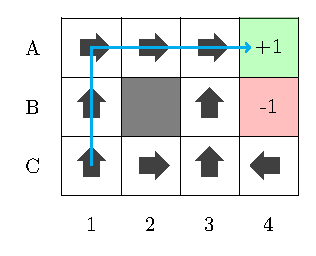
\includegraphics[]{gridworld/gridworld_tdl.pdf}
   \end{minipage}%
   \begin{minipage}[c]{.5\textwidth}
    $V(A3) \leftarrow V(A3)+ \alpha[R+\gamma V(A4)-V(A3)]\\
V(A3) = 0+0,1[-0,1+0,9 \cdot 1-0]=0,1$
   \end{minipage}
   \caption[\acs{TD} Update am Beispiel von Gridworld]{\acs{TD} Update am Beispiel von Gridworld. Der blaue Pfad zeigt den Pfad es Agenten in der ersten Episode. Rechts wird das \ac{TD} Update für den Zustand A3 berechnet. \protect\footnotemark}
   \label{fig:gridworld_tdl}
\end{figure}
\footnotetext{eigene Darstellung in Anlehnung an \cite[S. 99]{kontesg.SeminarReinforcementLearning2021}}
\subsection{\sarsa}
Der \ac{TD} Algorithmus Sarsa verwendet das Konzept von \ac{TD} Prediction, um die optimale Policy $\pi_*$ zu ermitteln. 
Statt der State-Value Funktion $v_\pi$ approximiert Sarsa die Action-Value Funktion $q_\pi$. 
Der Schätzwert der Action-Value Funktion $q_\pi$ ist $Q$. \cite[S. S. 129]{suttonReinforcementLearningIntroduction2018}
Die Action-Value Funktion $q_\pi(s,a)$ weist \ac{SA Tupel} einen \qValue zu. 
Der \qValue ist der kumulierte Reward, den der Agent erwarten kann, wenn er im Zustand $s$ die Aktion $a$ wählt und danach der Policy $\pi$ folgt. 
Für die Action-Value Funktion gilt daher auch die Beziehung aufeinander folgender Returns, sodass das \ac{TD} Update wie folgt formuliert werden kann \cite[S. 129f.]{suttonReinforcementLearningIntroduction2018}:

\begin{equation}
    \label{eq:sarsa_update}
    \equationentry{TD Update Sarsa}
    Q(S_t,A_t) \leftarrow Q(S_t,A_t) +\alpha[R_{t+1} + \gamma Q(S_{t+1},A_{t+1})-Q(S_t,A_t)]
\end{equation}

Um das Update durchführen benötigt Sarsa das Tupel $(S_t,A_t,R_{t+1},S_{t+1},A_{t+1})$, was der Ursprung für den Namen des Algorithmus ist. 
Auf Basis der Update-Regel kann Sarsa eine Schätzung $Q$ der Action-Value Funktion zur Policy $\pi$ aufstellen, nach der Sarsa mit der Umgebung interagiert. \cite[S. 129f.]{suttonReinforcementLearningIntroduction2018}
Der Agent verwaltet die Abbildung von \ac{SA Tupel} auf ihren geschätzten \qValue in einer \qtable. 
Mittels dieser kann Sarsa für jeden Zustand die Aktion ermitteln, die im höchsten \qValue resultiert.
Da Sarsa die \qValues mit jeder neuen Episode aktualisiert, kann Sarsa zur Interaktion mit der Umgebung einer Greedy-Policy folgen.
Bei einer Greedy-Policy wird immer die Aktion gewählt, die den höchsten \qValue hat.\footnote{Gibt es mehrere Aktionen mit dem höchsten\qValue, wird willkürlich eine der Aktionen gewählt}
Dadurch wird iterativ die Action-Value Funktion verbessert und die Policy nähert sich optimalen Policy $\pi_*$. \cite[S. 129f.]{suttonReinforcementLearningIntroduction2018}

Würde Sarsa ausschließlich gemäß einer Greedy-Policy mit der Umgebung interagieren, könnte der Agent in lokalen Maxima verweilen und würde nicht die optimale Policy lernen. 
Eine mögliche Lösung ist die $\epsilon$-greedy-Policy. 
Die $\epsilon$-greedy-Policy wählt mit einer Wahrscheinlichkeit von $\epsilon$ eine zufällige Aktion und $1-\epsilon$ die Aktion mit dem höchsten \qValue.
Der Hyperparameter $\epsilon$ ist die Explorationswahrscheinlichkeit. \cite[S. 28f.]{suttonReinforcementLearningIntroduction2018}

Damit Sarsa zur optimalen Policy $\pi_*$ konvergiert, muss neben den Konvergenzbedingungen von TD Prediction das Epsilon während dem Training gegen 0 konvergieren \cite[S. 129]{suttonReinforcementLearningIntroduction2018}. 
Bei der Wahl der Explorationswahrscheinlichkeit $\epsilon$ muss eine Balance zwischen Exploration und Exploitation, \dahe Ausnutzung der Aktionen mit höchsten \qValue, ermittelt werden. 
Das Abwägen beider Aspekte wird als Explorations-Exploitations-Dilemma bezeichnet \cite[S. 3]{suttonReinforcementLearningIntroduction2018}.

Der Ablauf des Sarsa Algorithmus ist als Pseudocode formuliert in Algorithmus \ref{algo_sarsa}.\footnote{eigene Darstellung in Anlehnung an \cite[S. 130]{suttonReinforcementLearningIntroduction2018}}

{\centering
\begin{minipage}{0.7\textwidth}
\begin{algorithm}[H]
\SetAlgoLined
\DontPrintSemicolon
\SetKwInput{kwAlgorithmParam}{Algorithm parameters}
\kwAlgorithmParam{step size $\alpha \in (0;1]$, small $\epsilon > 0$}
Initialize $Q(s,a)$, for all $s \in S^+, a \in A(s)$, arbitrarily except that $Q(terminal,\cdot)=0$\;
\BlankLine
\ForEach{episode}{
    Initialize $S$\;
    Choose $A$ from $S$ using policy derived from $Q$ (e.g., $\epsilon$-greedy)\;
    \ForEach{step of episode}{
        Take action $A$, observe $R$, $S'$\;
        Choose $A'$ from $S'$ using policy derived from $Q$ (e.g., $\epsilon$-greedy)\;
        $Q(S,A) \leftarrow Q(S,A) + \alpha[R+\gamma Q(S',A')-Q(S,A)]$\;
        $S \leftarrow S'; A \leftarrow A';$
    }
}
\caption{Sarsa}
\label{algo_sarsa}
\end{algorithm}
\end{minipage}
\par
}
\subsection{\qlearning}
Q-Learning lernt ebenfalls die optimale Policy durch Schätzung der Action-Value Funktion. 
Im Gegensatz zu Sarsa approximiert Q-Learning jedoch direkt die optimale Action-Value Funktion $q_*$ und somit die optimale Policy $\pi_*$.
Dafür nutzt Q-Learning bei der Aktualisierung seines Schätzwertes $Q(S_t,A_t)$ immer die Aktion $a$ des Folgezustands $S_{t+1}$, die den maximalen $Q$-Value hat.   
Dies ist  unabhängig davon welche Aktion $A_{t+1}$ der Agent schlussendlich ausführt.  \cite[S. 177]{watkinsLearningDelayedRewards1989} 
Das Update für Q-Learning kann daher wie in \cref{eq:ql_update} formuliert werden\cite[S. 131]{suttonReinforcementLearningIntroduction2018}.

\begin{equation}
    \label{eq:ql_update}
    \equationentry{TD Update Sarsa}
    Q(S_t,A_t)\leftarrow Q(S_t,A_t)+\alpha[R_{t+1}+\gamma\max_aQ(S_{t+1},a)-Q(S_t,A_t)]
\end{equation}

Die Policy $\pi$, die zur Interaktion mit der Umgebung genutzt wird, ist jedoch dennoch wichtig, da sie entscheidet welche Samples der Agent erhält. 
Da für die Aktualisierung jedoch immer der maximale Q-Value genutzt wird, ist eine Abnahme der Explorationswahrscheinlichkeit bei Nutzung von $\epsilon$-greedy keine Bedingung für die Konvergenz zur optimalen Policy \cite[S. 131f.]{suttonReinforcementLearningIntroduction2018}.
Wenn die Konvergenzbedingungen von \ac{TD} Prediction eingehalten werden, ist Q-Learning garantiert zur optimalen Policy $\pi_*$ zu konvergieren \cite[S. 286]{watkinsQlearning1992}.

Der Ablauf des Q-Learning Algorithmus ist als Pseudocode formuliert in Algorithmus \ref{algo_qlearning}.\footnote{eigene Darstellung in Anlehnung an \cite[S. 131]{suttonReinforcementLearningIntroduction2018}}

{\centering
\begin{minipage}{0.7\textwidth}
\begin{algorithm}[H]
\SetAlgoLined
\DontPrintSemicolon
\SetKwInput{kwAlgorithmParam}{Algorithm parameters}

\kwAlgorithmParam{step size $\alpha \in (0;1]$, small $\epsilon > 0$}
Initialize $Q(s,a)$, for all $s \in S^+, a \in A(s)$, arbitrarily except that $Q(terminal,\cdot)=0$\;
\BlankLine
\ForEach{episode}{
    Initialize $S$\;
    \ForEach{step of episode}{
        Choose $A$ from $S$ using policy derived from $Q$ (e.g., $\epsilon$-greedy)\;
        Take action $A$, observe $R$, $S'$\;
        $Q(S,A) \leftarrow Q(S,A) + \alpha[R+\gamma \max_{a} Q(S',a)-Q(S,A)]$\;
        $S \leftarrow S'$
    }
}
\caption{Q-Learning}
\label{algo_qlearning}
\end{algorithm}
\end{minipage}
\par
}



\subsection{Vergleich von \bothAlgs}
\label{chap:vergleich}

Die Algorithmen \bothAlgs haben zwei zentrale Unterschiede. 
Zum einen die Aktion des Folgezustands und somit der Q-Value, der für das Update genutzt wird. 
Zum anderen der Zeitpunkt, zu dem das Update durchgeführt wird \cite{IrelandComparisonThereFundamental}. 
Sarsa nutzt für das Update die Aktion, die es gemäß seiner Policy auswählt. 
Hingegen nutzt Q-Learning für das Update immer die Aktion mit dem höchsten Q-Value, auch wenn es gemäß Policy eine andere Aktion ausführt. 
Aufgrund dessen wird Sarsa als ein On-Policy und Q-Learning als ein Off-Policy Algorithmus klassifiziert \cite[S. 132]{suttonReinforcementLearningIntroduction2018}.

Zur Veranschaulichung des Unterschiedes wird das Update von Sarsa und Q-Learning am Beispiel von Gridworld erklärt. 
\cref{fig:gridworld_sample} zeigt die $\epsilon$-greedy-Policy, nach der beide Agent mit der Umgebung interagieren. 
Die State-Transition Probability und Rewardfunktion sind unverändert, aber den Agenten nicht bekannt.
Es gilt $\gamma=0,9$ und $\alpha=0,1$.
Der blaue Pfeil zeigt den Pfad einer Episode für beide Agenten. 
\cref{tab:tdlexample} enthält einen Ausschnitt einer willkürlich gefüllten Q-Tabelle für die Zustände C1 und C2.

\begin{minipage}{\textwidth}
  \begin{minipage}[b]{0.49\textwidth}
    \centering
    \captionsetup{type=figure}
    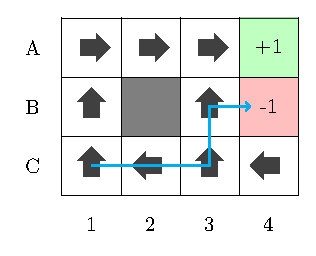
\includegraphics[]{gridworld/gridworld_sample.pdf}
    \captionof{figure}[Sample Episode für Gridworld]{Sample Episode für Gridworld\protect\footnotemark}
    \label{fig:gridworld_sample}
  \end{minipage}
  \hfill
  \begin{minipage}[b]{0.49\textwidth}
    \centering
    \captionsetup{type=table}
    % \begin{table}
\begin{tabular}{llr}
\toprule
Zustand $S$ & Aktion $A$    & $Q(S,A)$ \\ \midrule
C1          & Norden        & 10,5     \\
            & Westen        & 5,0      \\
            & Süden         & 8,7      \\
            & Osten         & 0,1      \\ \cmidrule{1-3}
C2          & Norden        & 8,2      \\ 
            & Westen        & -2,0     \\
            & Osten         & 9,8      \\
            & Süden         & 6,5      \\ \bottomrule
\end{tabular}
% \end{table}
% \begin{table}
% \centering
% \caption{\qtable mit Beispieleinträgen für Gridworld}
% \label{tab:qtable_tdl_example}

% \begin{tabular}{llr}
% \toprule
% Zustand $S$ & Aktion $A$    & $Q(S,A)$ \\ \midrule
% C1          & Norden        & 10,5     \\
%             & Westen        & 5,0      \\
%             & Süden         & 8,7      \\
%             & Osten         & 0,1      \\ \cmidrule{1-3}
% C2          & Norden        & 8,2      \\ 
%             & Westen        & -2,0     \\
%             & Osten         & 9,8      \\
%             & Süden         & 6,5      \\
% $\vdots$    & $\vdots$      & $\vdots$ \\ \bottomrule
% \end{tabular}
% \end{table}
    \captionof{table}{Willkürlich gefüllte \qtable für Gridworld}
    \label{tab:tdlexample}
    \end{minipage}
\end{minipage}
\footnotetext{eigene Darstellung in Anlehnung an \cite[S. 127]{kontesg.SeminarReinforcementLearning2021}}

Im Zustand C1 wählt der Agent die Greedy-Aktion “Norden”. Wegen der Transposition-Probability wechselt der Agent jedoch in den Zustand C2. Im Zustand C2 ist die Greedy-Aktion “Osten”. Der Agent wählt aufgrund von $\epsilon$-greedy zufällig die Aktion “Westen”. Das Sample $(S_t,A_t,R_{t+1},S_{t+1},A_{t+1})$ der Umgebung ist somit: $(C1;N;-0,1;C2;W)$ 

Der Sarsa-Agent führt das Update in \cref{eq:sarsa_update_example} durch. Hingegen wählt der Q-Learning Agent für den Folgezustand die Aktion mit höchstem Q-Value $Q(C2,Osten)=9,8$ führt daher das Update aus \cref{eq:ql_update_example} durch.

\begin{equation}
    \label{eq:sarsa_update_example}
    \equationentry{Beispiel TD Update Sarsa}
    \begin{split}
    Q(C1,N) & =Q(C1,N)+\alpha[-0,01+0,09Q(C2, W)-Q(C1,N)] \\
    Q(C1,N) & =10,5+0,1[-0,1+0.9(-2,0)-10.5]=9,26
    \end{split}
\end{equation}

\begin{equation}
    \label{eq:ql_update_example}
    \equationentry{Beispiel TD Update Q-Learning}
    \begin{split}
        Q(C1,N) &=Q(C1,N)+\alpha[-0,01+0,09Q(C2, O)-Q(C1,N)]\\
        Q(C1,N) &=10,5+0,1[-0,1+0.9(9,8)-10.5]=10,32
    \end{split}
\end{equation}



Würden beide Algorithmen einer Greedy-Policy folgen, wäre das Update gleich. 
Während Sarsa seine Aktion $A_{t+1}$ vor dem Update ausgewählt hat, wählt Q-Learning diese erst, nachdem das Update durchgeführt wurde. 
In Situationen, in denen ein Zustand der eigene Folgezustand ist, könnten Q-Learning und Sarsa unterschiedliche Aktionen $A_{t+1}$ auswählen, da sich die \qValues der Aktionen durch das Update geändert haben könnten. \cite{IrelandComparisonThereFundamental}

Ein weiteres Beispiel, dass den Unterschied von Q-Learning und Sarsa verdeutlicht ist \gqq{Cliff Walking} in \cref{fig:cliffwalking}. 
Bei diesem soll ein Agent vom Startbereich “S” zum Ziel “G” laufen. 
In jedem Zeitschritt erhalten die Agenten einen Reward $-1$, sodass sie das Ziel möglichst schnell erreichen sollen. 
Betritt ein Agent den Bereich Klippe, erhält dieser einen Reward von $-100$. 
Die Agenten können sich wieder in alle vier Himmelsrichtungen bewegen. 
Im Gegensatz zur Gridworld sind die Zustandsübergänge deterministisch. 
Die Algorithmen Q-Learning und Sarsa lernen beide mittels einer $\epsilon$-greedy-Policy mit konstantem $\epsilon$=0,1. 
Die Abbildung zeigt den optimalen Pfad (rot) und den sicheren Pfad (blau), der einen geringeren Return erzielt, aber mit größerer Wahrscheinlichkeit im Ziel ankommt. 
Während des Trainings lernt Q-Learning den optimalen Pfad, betritt jedoch aufgrund von $\epsilon=0,1$ regelmäßig die Klippe. 
Hingegen lernt Sarsa den sicheren Pfad, da es im Update die aktuelle Policy beachtet. 
Konvergiert $\epsilon$ während dem Training gegen 0 lernt Sarsa ebenfalls den optimalen Pfad. \cite[S. 132]{suttonReinforcementLearningIntroduction2018}

\begin{figure}[h]
    \centering
    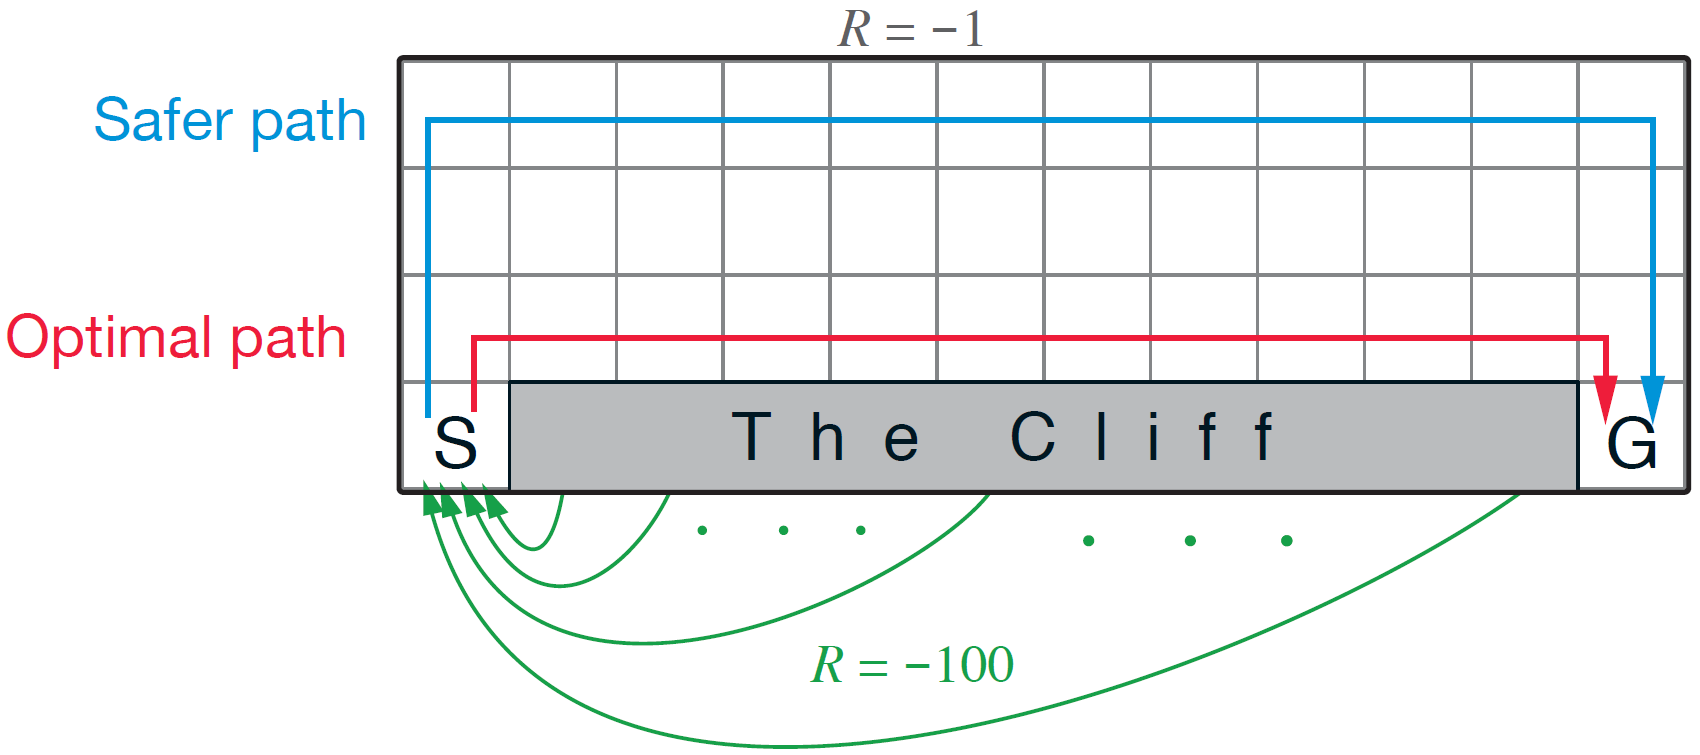
\includegraphics[scale=0.2]{04_Artefakte/01_Abbildungen/rl/rl_cliff_environment.png}
    \caption[Cliff Walking]{Cliff Walking\protect\footnotemark}
    \label{fig:cliffwalking}
\end{figure}
\footnotetext{Abbildung entnommen aus \cite[S. 132]{suttonReinforcementLearningIntroduction2018}}

Beide Algorithmen haben jedoch die gleichen Limitierungen. Da beide Algorithmen durch Interaktion mit der Umgebung lernen, werden hinreichend viele Samples benötigt, um die Action-Value Funktion zu approximieren. 
Zudem spielt die Wahl der Lernrate eine entscheidende Rolle für den Trainingserfolg. \cite[S. 131]{kontesg.SeminarReinforcementLearning2021}
Da für jedes \ac{SA Tupel} ein eigener Eintrag in der Q-Tabelle vorhanden sein muss, haben die Algorithmen zwei weitere Limitierungen.
Erstens, können beide Algorithmen nur für Probleme genutzt werden, bei denen eine Verwaltung der zu speichernden \ac{SA Tupel} praktikabel ist.
Zweitens können die Algorithmen nur optimale Entscheidungen treffen, wenn sie die \ac{SA Tupel} kennen. 
Eine Generalisierung der gesammelten Erfahrung auf neue Zustände ist nicht möglich. 
Um beide Limitierungen zu beheben können die Algorithmen mit neuronalen Netzten verknüpft werden.
Diese werden dann genutzt, um die \statevalueFunktion zu approximieren und so keine \ac{SA Tupel} speichern zu müssen und gesammelte Erfahrung zu generalisieren. \cite[S. 195f.]{suttonReinforcementLearningIntroduction2018}, \cite[S. 137ff.]{kontesg.SeminarReinforcementLearning2021}
\section{Minimax-Algorithmus}
\label{sec:minimax}
Jedes Zug-basierte Spiel kann als ein gerichteter Graph dargestellt werden, der als Spielbaum bezeichnet wird. 
Jeder Knoten im Spielbaum entspricht einem legalen Spielzustand.
Der Ausgangszustand des Spielfelds ist der sogenannte Wurzelknoten.  
Die Knoten sind verbunden durch Kanten, die die legalen Aktionen und somit Zustandsübergänge repräsentieren. 
Nehmen zwei Spieler abwechselnd Aktionen vor, entscheidet die Tiefe des Spielbaums ausgehend vom Wurzelknoten, welcher Spieler am Zug ist.   
Spielendzustände werden durch Terminalknoten repräsentiert, von denen keine weiteren Kanten ausgehen. \cite[S. 650f.]{millingtonArtificialIntelligenceGames2009}, \cite[S. 123 ff.]{russellArtificialIntelligenceModern2021} 

Jedem Terminalknoten \bzw Spielergebnis kann mittels einer Bewertungsfunktion ein Wert zugewiesen werden. 
Dieser wird als Utility bezeichnet und ist abhängig von der Art des Spiels, das der Baum repräsentiert.
Ein solcher Baum kann zur Darstellung eines Nullsummenspiels genutzt werden. \cite[S. 650f.]{millingtonArtificialIntelligenceGames2009}, \cite[S. 123 ff.]{russellArtificialIntelligenceModern2021} 
Ein Nullsummenspiel, wie beispielsweise Tic-Tac-Toe oder Schach, ist ein Spiel, bei dem der Gewinn des einen Spielers ein Verlust für die anderen Spieler bedeutet \cite[S. 6]{allisSearchingSolutionsGames1994}. Somit gibt es zwei äquivalente Möglichkeiten das Ziel jedes Spielers ausdrücken: Ein Spieler versucht zu gewinnen \bzw dafür zu sorgen, dass der Gegner verliert.
Als Utility wird bei Zweispieler-Nullsummenspielen üblicherweise der Wert $+1$ für den Sieg des beginnenden Spielers und $-1$ für den Sieg des nachziehenden Spielers genutzt.
Ein Unentschieden hat die Utility $0$ \cite[S. 649ff.]{millingtonArtificialIntelligenceGames2009}, \cite[S. 123 ff.]{russellArtificialIntelligenceModern2021}

Werden die Ziele der Spieler auf Basis der Utility formuliert, so versucht der beginnende Spieler die Utility zu maximieren, \dahe das Spiel mit $+1$ zu beenden. Der nachziehende Spieler möchte, dass der Gegner verliert und somit die Utility minimieren, \dahe das Spiel soll mit mit $-1$ enden.
Geht man von zwei optimalen Spielern aus, werden diese in jedem Knoten entsprechend die Aktion wählen, die die Utility maximiert oder minimiert. \cite[S. 124]{russellArtificialIntelligenceModern2021}
Dieser Sichtwechsel zwischen Maximieren und Minimieren bildet die Grundlage des Minimax-Algorithmus. \cite[S. 655]{millingtonArtificialIntelligenceGames2009}
Der Minimax-Algorithmus basiert auf dem Minimax-Theorem der Spieltheorie \cite{v.neumannZurTheorieGesellschaftsspiele1928} und wurde erstmals 1950 in \cite{shannonXXIIProgrammingComputer1950} für Schach formuliert. 
Es ist ein Verfahren um in Spielbäumen von Zweispieler-Nullsummenspielen die optimale Aktion zu finden, unter der Annahme, dass der Gegner ebenfalls seine optimale Aktion wählt \cite[S. 7]{shannonXXIIProgrammingComputer1950}. 

Minimax ist ein rekursiver depth-first (\dt Tiefensuche) Algorithmus, der im Wurzelknoten beginnt. 
Je nach Rolle \bzw Tiefe des Knoten, wird die minimale oder maximale Utility des Kindknoten und die dafür notwendige Aktion übernommen. 
Dafür betrachtet der Algorithmus die Utility aller Kindknoten. 
Da nur Terminalknoten eine Utility durch die Bewertungsfunktion zugewiesen wird, werden solange die Kindknoten jedes Knoten betrachtet, bis die Terminalknoten erreicht wurden. 
Der Elternknoten übernimmt dann die Utility des Kindknoten mit dem minimalen oder maximalen Wert, sodass der darüber liegende Knoten die zu erwartende Utility erhält und wählen kann. \cite[S. 123ff.]{russellArtificialIntelligenceModern2021}, \cite[S. 654ff.]{millingtonArtificialIntelligenceGames2009}
Dieser Prozess ist visualisiert in \cref{fig:minimax_example} und als Pseudocode beschrieben in Algorithmus \ref{algo_minimax}.

\begin{figure}
    \centering
    \begin{subfigure}[b]{0.45\textwidth}
      \centering
      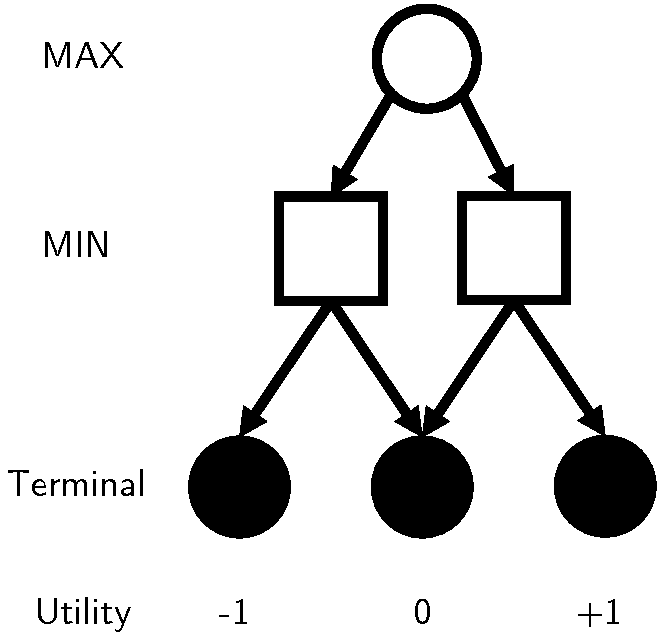
\includegraphics[scale=0.3]{minimax/minimax_step0.pdf}
      \caption{Spielbaum im Ausgangszustand}
      \label{fig:minimax_step0}
    \end{subfigure}
    \begin{subfigure}[b]{0.45\textwidth}
      \centering
      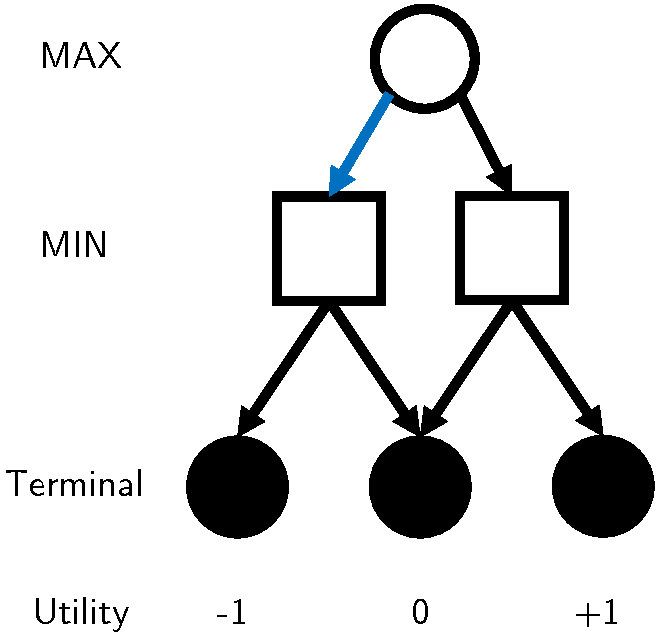
\includegraphics[scale=0.3]{minimax/minimax_step1.pdf}
      \caption{MAX prüft Utility der Kindknoten}
      \label{fig:minimax_step1}
    \end{subfigure}
    \begin{subfigure}[b]{0.45\textwidth}
      \centering
      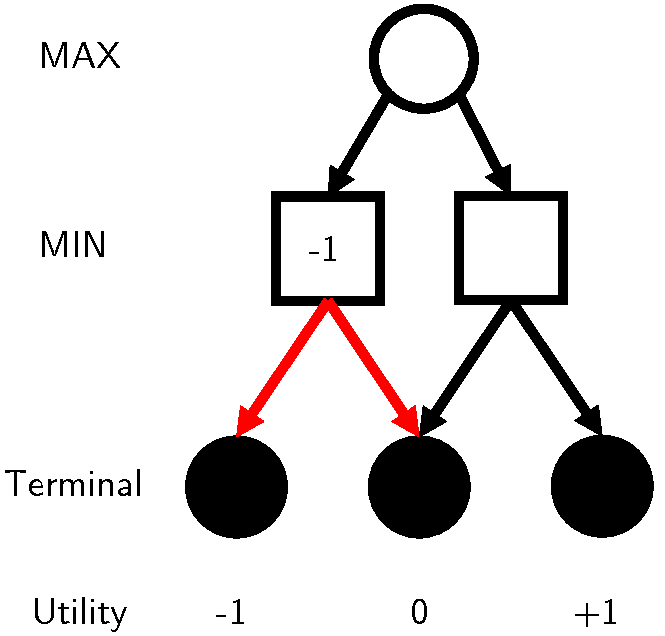
\includegraphics[scale=0.3]{minimax/minimax_step2.pdf}
      \caption{MIN prüft Utility der Terminalknoten und übernimmt kleinste Utility}
      \label{fig:minimax_step2}
    \end{subfigure}
    \begin{subfigure}[b]{0.45\textwidth}
      \centering
      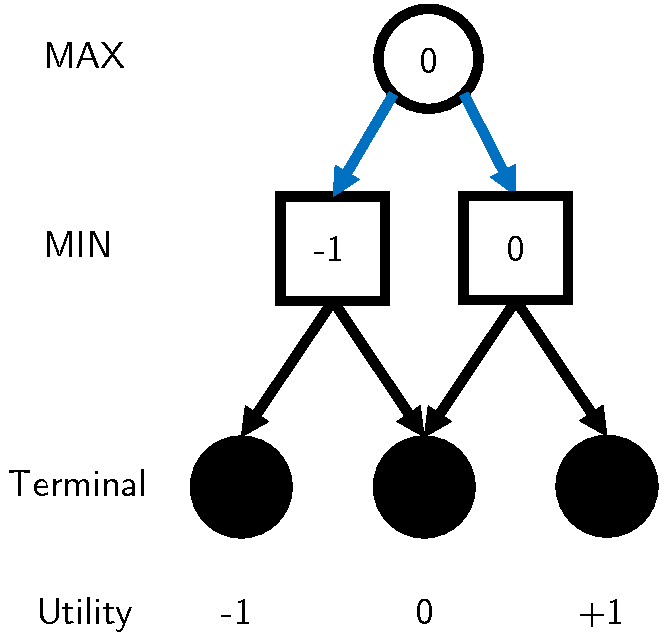
\includegraphics[scale=0.3]{minimax/minimax_step3.pdf}
      \caption{b) und c) werden für rechte Seite wiederholt und MAX wählt größte Utility aus}
      \label{fig:minimax_step3}
    \end{subfigure}
    \caption[Visualisierung des Minimax-Algorithmus]{Visualisierung des Minimax-Algorithmus für ein fiktives Zweispieler-Nullsummenspiel in vier Schritten. Knoten des maximierenden Spielers (MAX) sind Kreise, Knoten des minimierenden Spielers (MIN) Quadrate.}
    \label{fig:minimax_example}
\end{figure}

{\centering
\begin{minipage}{0.60\textwidth}
\begin{algorithm}[H]
\SetAlgoLined
\DontPrintSemicolon
\SetKwFunction{KwMinimax}{Minimax}
\SetKwProg{Fn}{Function}{:}{}
\Fn{\KwMinimax{NODE, PLAYER}}{
    \uIf{NODE is terminal}{
        \KwRet{utility assigned to NODE}
    }
    \uElseIf{PLAYER is maximizing player MAX}{
        \ForEach{child of NODE}{
            \KwMinimax{CHILD, MIN}\;
        }
        \KwRet{maximal CHILD utility}
    }
    \Else{
        \ForEach{child of NODE}{
            \KwMinimax{CHILD, MAX}\;
        }
        \KwRet{minimal CHILD utility}
    }
}
\textbf{end function}

\caption{Pseudocode Minimax-Algorithmus}
\label{algo_minimax}
\end{algorithm}
\end{minipage}
\par
}


Da manche Knoten in Spielbäumen durch unterschiedliche Zugfolgen erreicht werden können, kann der Minimax-Algorithmus durch eine Transposition table (\dt Zugumstellungs-Tabelle) erweitert werden.
Bei diesen werden Informationen zu Knoten in einer Lookup-Tabelle hinterlegt, sodass direkt auf diese zugegriffen werden kann. \cite[S. 651]{millingtonArtificialIntelligenceGames2009}, \cite[S. 22]{slateCHESSNorthwesternUniversity1983}, \cite[S. 807]{greenblattGreenblattChessProgram1988}
Der Name Transposition table leitet sich vom Schach ab, bei dem unterschiedliche Spielzüge, um einen gleichen Zustand zu erreichen, als Transposition (dt. Zugumstellung) bezeichnet werden \cite[S. 651]{millingtonArtificialIntelligenceGames2009}. 
Andere Vereinfachungen und Erweiterungen des Minimax-Algorithmus, wie beispielsweise \gqq{Negamax} oder Alpha-Beta-Pruning \cite[S. 115]{ertelIntroductionArtificialIntelligence2017} werden in dieser Arbeit nicht betrachtet.


\section{Tic-Tac-Toe}

In diesem Abschnitt wird das Strategiespiel Tic-Tac-Toe (\ac{TTT}) erklärt. Anschließend wird begründet, wieso die vorgestellten Algorithmen darauf angewandt werden können. 

\subsection{Spielerklärung}
\acl{TTT} ist ein Strategiespiel, das von zwei Spielern gespielt wird \cite[S. 6]{allisSearchingSolutionsGames1994}.
Das Spielfeld ist unterteilt in neun Bereiche (Slots), die in einer 3x3 Matrix angeordnet sind. 
%Die Slots gehören daher zu einer von drei Klassen, die als Ecken, Kanten oder Mitte bezeichnet werden. Zu Beginn sind alle Slots leer. 
Die Spieler platzieren abwechselnd ihr zugeteiltes Symbol, entweder X oder O, in einem Slot auf dem Spielfeld. 
Der beginnende Spieler verwendet in der Regel das Symbol X. 
Ziel jedes Spielers ist es, drei eigene Symbol entweder vertikal, horizontal oder diagonal in einer Reihe zu platzieren.
Somit gibt es insgesamt acht mögliche Gewinnkonstellationen: drei Zeilen, drei Spalten und zwei Diagonalen. 
Sind alle Slots belegt ohne, dass einer der Spieler gewonnen hat, endet das Spiel in einem Unentschieden. \cite[S. 533]{crowleyFlexibleStrategyUse1993}

\acs{TTT} besitzt 5478 legale Spielfeldkonstellationen und hat im Vergleich zu Spielen wie Schach oder Vier Gewinnt eine deutlich geringere Zustandsraum-Komplexität  \cite[S. 159]{allisSearchingSolutionsGames1994}.
Dies kann sogar weiter reduziert werden, da aufgrund von Rotations- und Spiegelsymmetrien bis zu acht Spielfeldkonstellationen äquivalent sein können.\footnote{4 Rotationen und 4 Spiegelungen, jeweils horizontal/vertikal mit und ohne 90° Drehung} 
Dadurch reduziert sich die Zustandsraum-Komplexität auf 765. \cite[S. 3]{block-berlitzm.ProInformatikFunktionaleProgrammierung2009}

In der Spieltheorie ist \acs{TTT} ein klassisches Beispiel für ein Nullsummenspiel, da ein Gewinn immer mit einer Niederlage für den Gegner einhergeht \cite[S. 6]{allisSearchingSolutionsGames1994}, \cite[S. 533]{crowleyFlexibleStrategyUse1993}.
Zudem gehört TTT zu den Spielen mit perfekter Information, weil beide Spieler Zugriff auf alle Informationen des aktuellen Spielzustands haben \cite[S. 156]{allisSearchingSolutionsGames1994}, \cite[S. 38]{gardnerm.HexaflexagonsOtherMathematical1988}.
\acs{TTT} ist ein stark gelöstes Spiel, \dahe es gibt eine optimale Strategie für jede legale Position \cite[S. 6]{allisSearchingSolutionsGames1994}
Spielen beide Spieler optimal endet TTT immer in einem Unentschieden und wird daher als futile Game (\dt vergebliches Spiel) bezeichnet \cite[S. 177]{wangPopularLecturesMathematical2014}.
Somit ist das beste Spielergebnis immer zu Gewinnen und gegen einen optimalen Spieler Unentschieden zu spielen. 
Regeln für ein perfektes Spiel wurden erstmals 1972 in \cite{newellHumanProblemSolving1972} formuliert. 
\citeauthor{crowleyFlexibleStrategyUse1993} erweiterten diese unter der Bezeichnung \gqq{Model of Expert Performance}, wie im Anhang \cref{chap:ModelofExpert} gelistet \cite[S. 536]{crowleyFlexibleStrategyUse1993}. 
Die folgenden vier Regeln \bzw Aktionen bilden in der dargestellten Reihenfolge die zentrale Strategie für Expert Play. Beispielhafte Spielfeldkonstellationen werden in Abbildung \cref{fig:ttt_expertplay} gezeigt.

\begin{enumerate}
    \item \textbf{Win}: Wenn der Spieler eine Möglichkeit hat zu gewinnen, soll diese genutzt werden
    \item \textbf{Block}: Wenn der Gegner zwei Symbole in einer Reihe hat, blockiere den Gewinn des Gegners
    \item \textbf{Fork}: Wenn sich zwei Reihen schneiden, in denen der Spieler sein Symbol platziert hat und der Slot, wo sie sich schneiden leer ist, belege diesen Slot
    \item \textbf{Block Fork}: Wenn die Möglichkeit besteht, zwei Symbole in eine Reihe zu legen, wähle diesen Slot, um den Gegner zum Blocken zu zwingen. Andernfalls wähle einen Slot, um ein Fork des Gegners zu verhindern
\end{enumerate}

\begin{figure}
    \centering
    \begin{subfigure}[b]{0.45\textwidth}
      \centering
      
\includegraphics[scale=0.7]{ttt_boards/ttt_win.pdf}
      \caption{Win}
      \label{fig:ttt_win}
    \end{subfigure}
    \begin{subfigure}[b]{0.45\textwidth}
      \centering
      
\includegraphics[scale=0.7]{ttt_boards/ttt_block.pdf}
      \caption{Block}
      \label{fig:ttt_block}
    \end{subfigure}
    \begin{subfigure}[b]{0.45\textwidth}
      \centering
      
\includegraphics[scale=0.7]{ttt_boards/ttt_fork.pdf}
      \caption{Fork}
      \label{fig:ttt_fork}
    \end{subfigure}
    \begin{subfigure}[b]{0.45\textwidth}
      \centering
      
\includegraphics[scale=0.7]{ttt_boards/ttt_blockfork.pdf}
      \caption{Block Fork}
      \label{fig:ttt_blockfork}
    \end{subfigure}
    \caption[Beispielhafte Spielfeldkonstellationen für TTT Expert Play]{Beispielhafte Spielfeldkonstellationen für \acs{TTT} Expert Play. Optimale Aktionen sind grau gefärbt \protect\footnotemark}
    \label{fig:ttt_expertplay}
\end{figure}

\footnotetext{Spielfeldkonstellationen übernommen aus \cite[S. 539]{crowleyFlexibleStrategyUse1993}, Alle \acs{TTT} Spielfelder werden erstellt mit Code von \cite{sebglavCreatingTicTacToeBoards2022}}

Der zweite Teil der Strategie beschäftigt sich mit dem optimalen ersten Zug für X. 
Aufgrund der Äquivalenz der möglichen Aktionen reduziert sich die Auswahl auf drei Möglichkeiten: Ecke, Kante und Mitte. 
In \cite[S. 38]{gardnerm.HexaflexagonsOtherMathematical1988} wird die Ecke als stärkste Aktion dargestellt, da der Gegner mit der Mitte kontern muss, um nicht zu verlieren. 
Hingegen zeigen Studien wie \cite{kutscheraa.BestOpeningMove2018}, dass die Mitte die beste Aktion ist, da diese in der Menge aller möglichen Spielabfolgen die Startposition mit den meisten gewonnen Spielen ist.
Spielen zwei optimale Spieler gegeneinander ist die Wahl der ersten Aktion unbedeutend \cite[S. 38]{gardnerm.HexaflexagonsOtherMathematical1988}.

\subsection{Anwendbare Algorithmen}
\label{sec:anwendbare_algorithmen}
Eine Voraussetzung für die Anwendung des Minimax-Algorithmus ist, dass der Spielbaum eine geringe Komplexität hat \cite[S. 10]{block-berlitzm.ProInformatikFunktionaleProgrammierung2009}.
Die Spielbaum-Komplexität ist definiert als die Anzahl der Terminalknoten des vollständig konstruierten Spielbaums und wird angegeben als $\log$ zur Basis $10$ \cite[S. 160]{allisSearchingSolutionsGames1994}.
Aufgrund des kleinen Zustands- und Aktionsraums von \ac{TTT}, ist dessen Spielbaum klein.
Die Spielbaum-Komplexität beträgt $5$ ist im Vergleich zu Spielen wie Schach (123) oder Shogi (226) relativ gering \cite[S. 11]{block-berlitzm.ProInformatikFunktionaleProgrammierung2009}.
Somit erfüllt \ac{TTT} diese Bedingung für die Anwendung des Minimax-Algorithmus.
Eine weitere Bedingung des Minimax-Algorithmus ist, dass das Spiel ein Zweispieler-Nullsummenspiel mit perfekter Information sein muss \cite[S. 10]{block-berlitzm.ProInformatikFunktionaleProgrammierung2009}. 
Da \ac{TTT} auch diese Bedingung erfüllt, kann der Minimax-Algorithmus angewendet werden.
In \cref{fig:ttt_tree} ist ein Auszug des Spielbaums von \acs{TTT} mit der möglichen Umsetzung eines Minimax-Algorithmus dargestellt. Jedoch ist anzumerken, dass der Minimax-Algorithmus einen optimalen Gegner erwartet und daher nur gegen diese optimal spielt. Minimax kann nicht verlieren, aber wählt seine Aktionen nicht, um seine Gewinnwahrscheinlichkeit gegen nicht optimale Spieler zu maximieren. \cite[S. 8]{suttonLearningPredictMethods1988}. 

Voraussetzung für die Anwendung von \ac{TDL} Algorithmen ist, dass das zu lösende Problem als \ac{MDP} formuliert werden kann.
Der mögliche Zustandsraum $S$ und Aktionsraum $A$ sind für \ac{TTT} diskret und bekannt. 
Da \ac{TTT} ein Spiel mit perfekter Information ist, kann bei gegebenem Zustand $s$ und Aktion $a$ der Folgezustand $s'$ bestimmt werden.
Somit erfüllt \ac{TTT} die Markov Eigenschaft und kann als ein \ac{MDP} modelliert werden.
Die weitere Voraussetzung ist, dass der Agent mit seiner Umgebung interagieren kann und von dieser Samples in Form des Tupels $(S_t,A_t,R_{t+1},S_{t+1})$ erhält. \cite[S. 88]{kontesg.SeminarReinforcementLearning2021}
Diese kann im Rahmen der Implementierung beachtet werden. 
Da somit beide Voraussetzungen erfüllt sind, können \ac{TDL} Methoden wie \bothAlgs angewendet werden.

\begin{figure}[h]
    \centering
    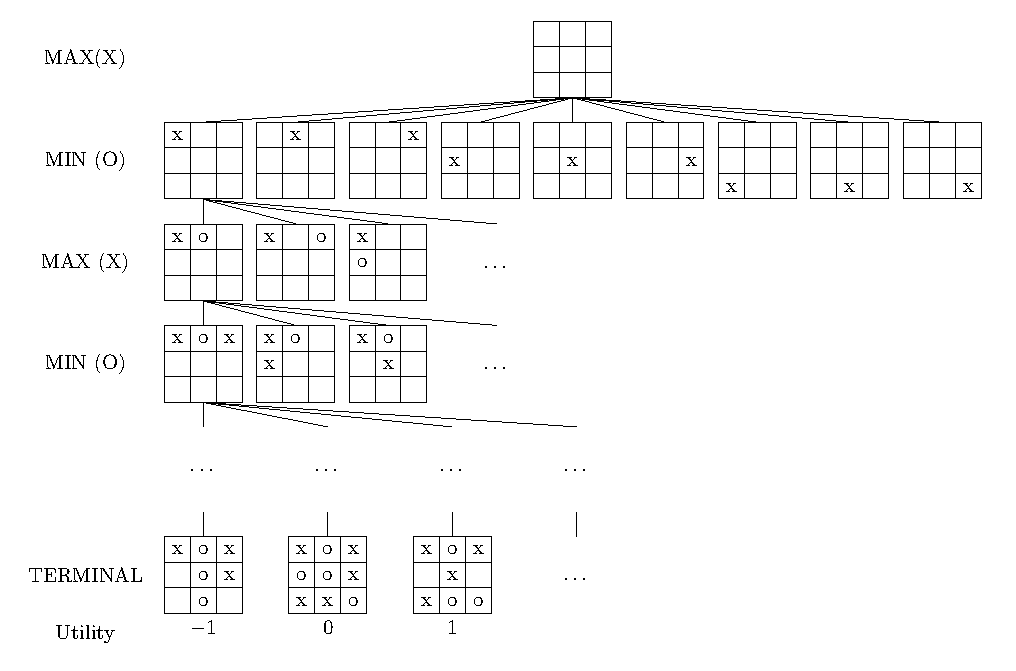
\includegraphics[scale=0.7]{04_Artefakte/01_Abbildungen/ttt_boards/ttt_tree.pdf}
    \caption[Auszug aus dem Spielbaum von \acs{TTT}]{Auszug aus dem Spielbaum von \acs{TTT} \protect\footnotemark}
    \label{fig:ttt_tree}
\end{figure}

\footnotetext{Darstellung übernommen aus \cite[S. 125]{russellArtificialIntelligenceModern2021}, Abbildung erstellt mit Code von \cite{vj.l.TikzPgfFollowup}}
